\chapter{Jupter Notebook语法}
\section{JupyterLab的语法指令}
\subsection{writefile 写到一个文件}
\begin{lstlisting}[style=demostyle,numbers=none]
%%writefile 文件名
内容
\end{lstlisting}  

将当前cell的内容写入到文件中。

\begin{figure}[htpb]
  \centering
  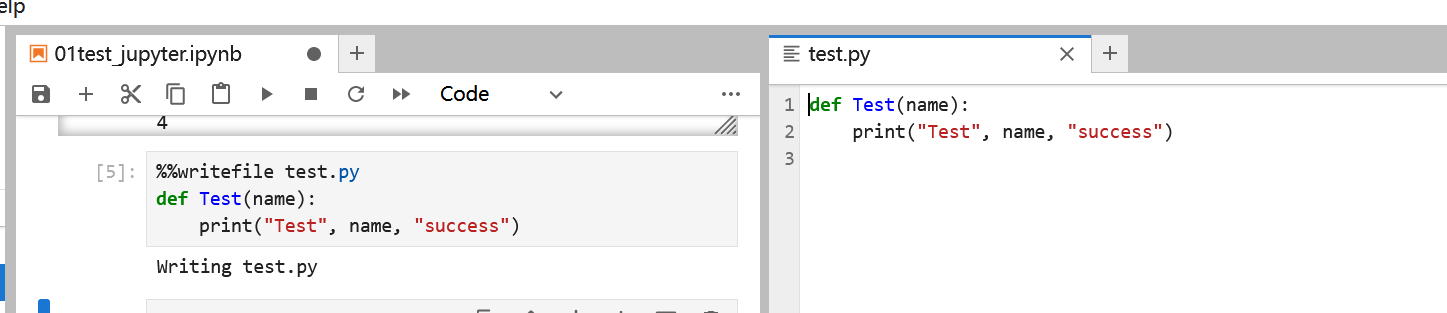
\includegraphics[width=0.6\textwidth]{part/软件工程/环境搭建/JupyterNotbook/pic/jupyternotebook语法/writefile指令.png}
  \caption{writefile指令}
  % \label{fig:writefile指令}
\end{figure}


\subsection{pycat 显示一个文件}
\begin{lstlisting}[style=demostyle,numbers=none]
%pycat 文件名
\end{lstlisting}

\begin{figure}[htpb]
  \centering
  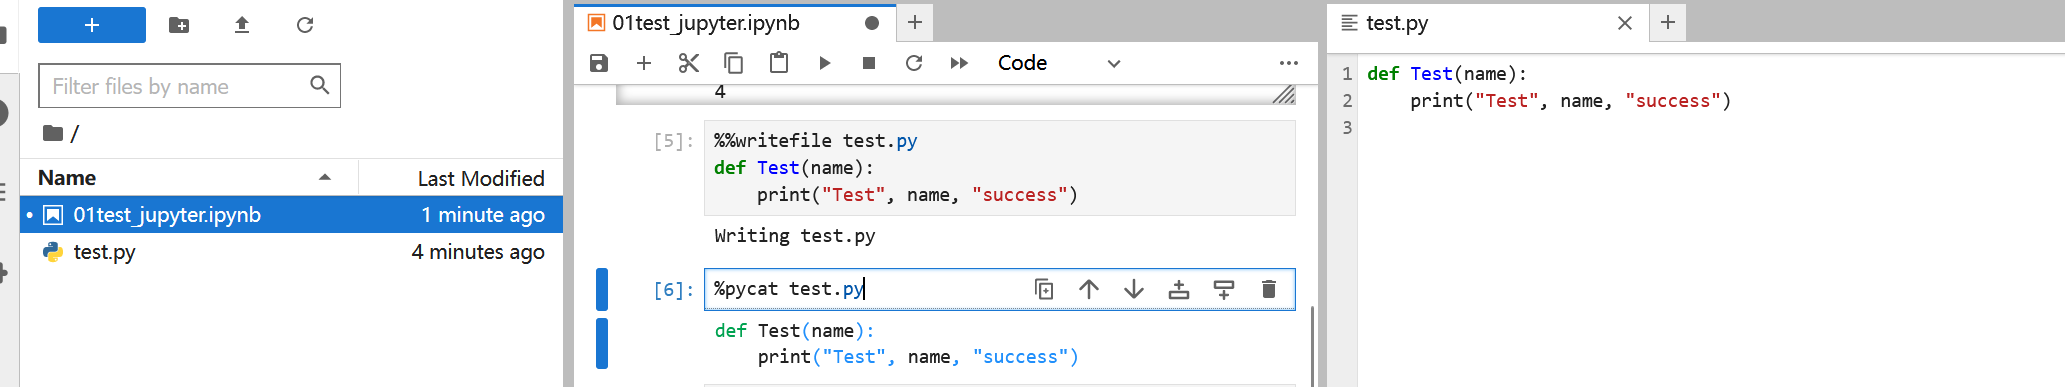
\includegraphics[width=0.6\textwidth]{part/软件工程/环境搭建/JupyterNotbook/pic/jupyternotebook语法/pycat指令.png}
  \caption{pycat指令}
  \label{fig:pycat指令}
\end{figure}


\subsection{run 执行一个文件}
\begin{lstlisting}[style=demostyle,numbers=none]
%run 文件名  
函数名(参数)
\end{lstlisting}

当然也可以通过\codeinline{import 文件名}导入文件,\codeinline{from 文件名 import 函数名}导入函数。

\begin{figure}[htpb]
  \centering
  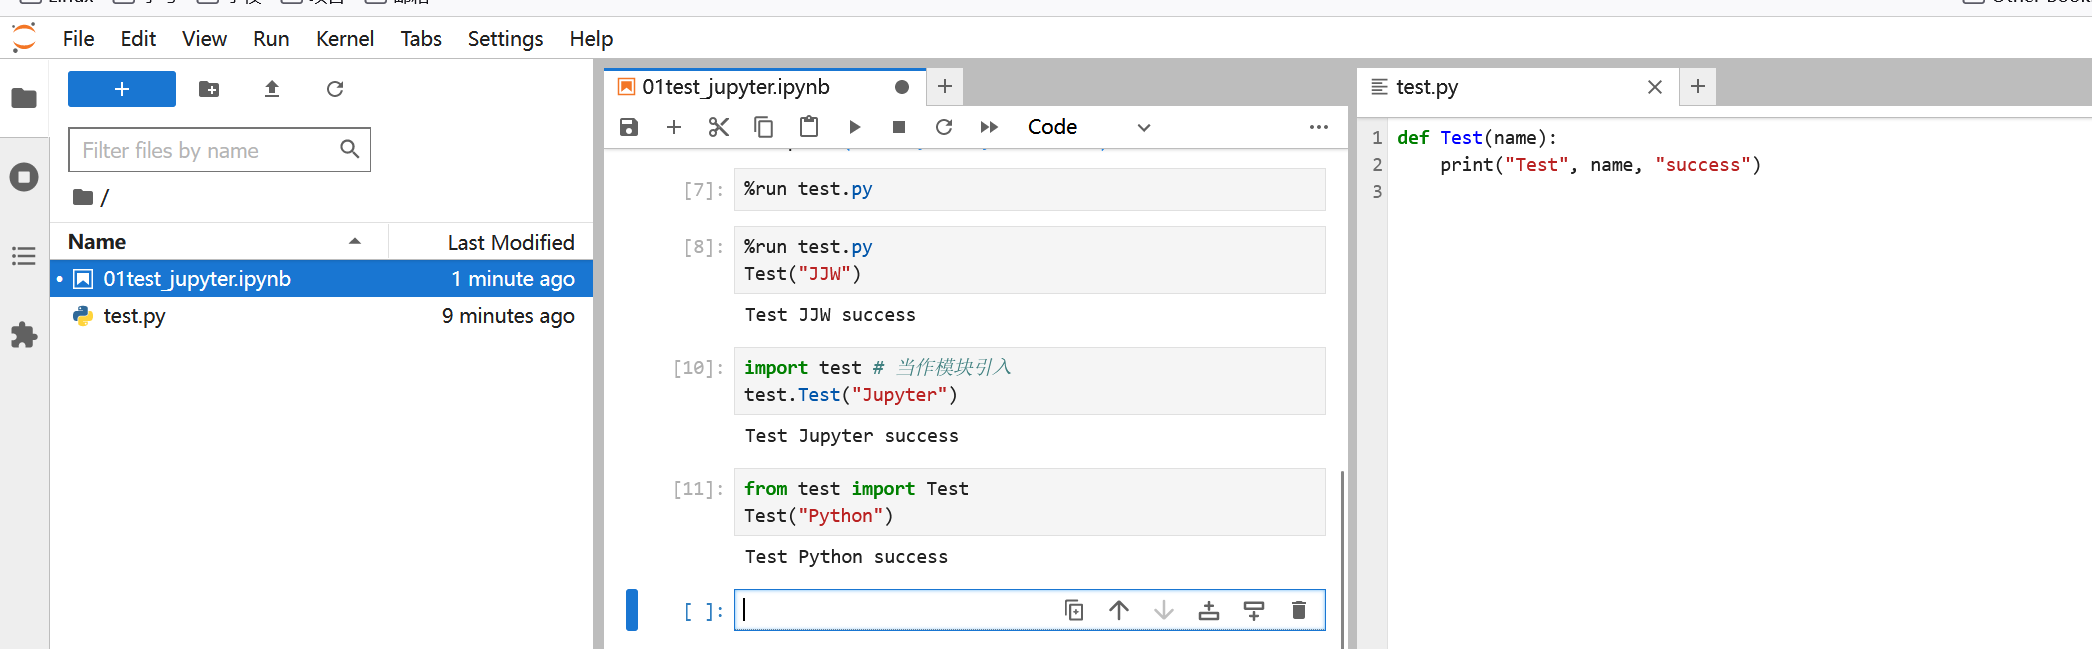
\includegraphics[width=0.6\textwidth]{part/软件工程/环境搭建/JupyterNotbook/pic/jupyternotebook语法/run指令.png}
  \caption{run指令}
  \label{fig:run指令}
\end{figure}

\subsection{计算代码运行时间}
多轮测试，取平均值。
\begin{lstlisting}[style=demostyle,numbers=none]
%timeit 函数名(参数) # 测试一条语句的运行时间

%%timeit # 测试一个cell的运行时间
\end{lstlisting}

只测试一次。
\begin{lstlisting}[style=demostyle,numbers=none]
%time 函数名(参数) # 测试一条语句的运行时间

%%time # 测试一个cell的运行时间
\end{lstlisting}

\begin{figure}[htpb]
  \centering
  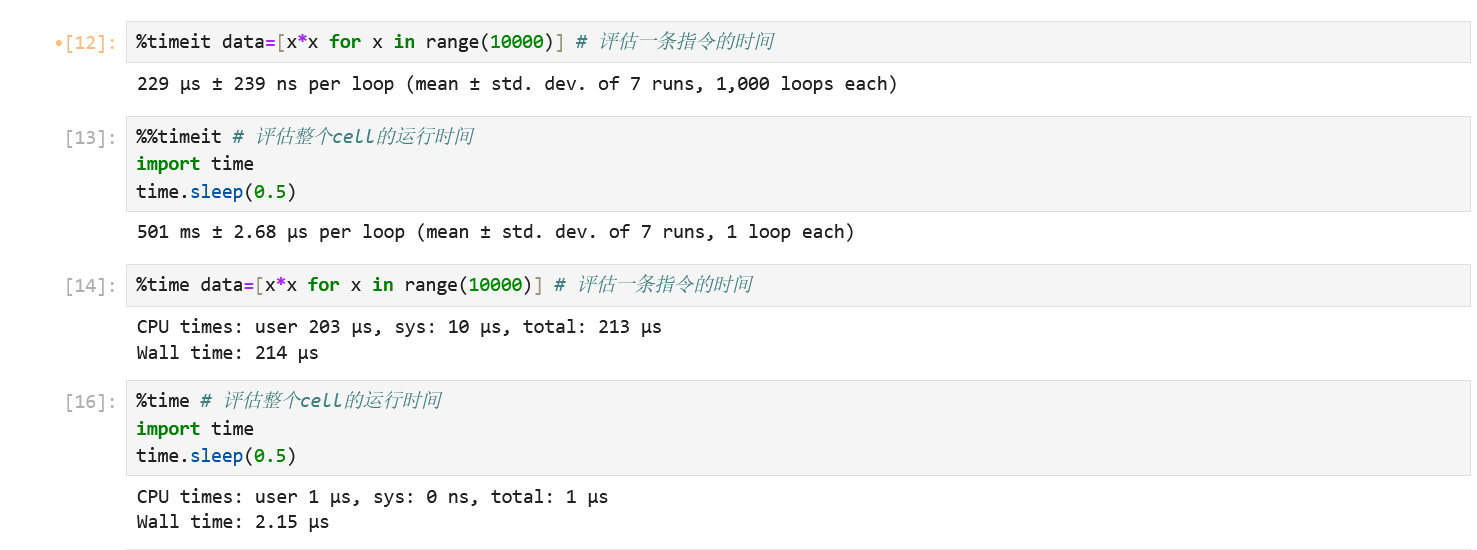
\includegraphics[width=0.6\textwidth]{part/软件工程/环境搭建/JupyterNotbook/pic/jupyternotebook语法/timeit和time指令.png}
  \caption{timeit和time指令}
  \label{fig:timeit和time指令}
\end{figure}

\subsection{whos 查看当前内存中的变量}
使用\codeinline{\%whos}或者\codeinline{\%who}查看当前内存中的变量。

包括定义的变量、函数、模块等。

\begin{figure}[htpb]
  \centering
  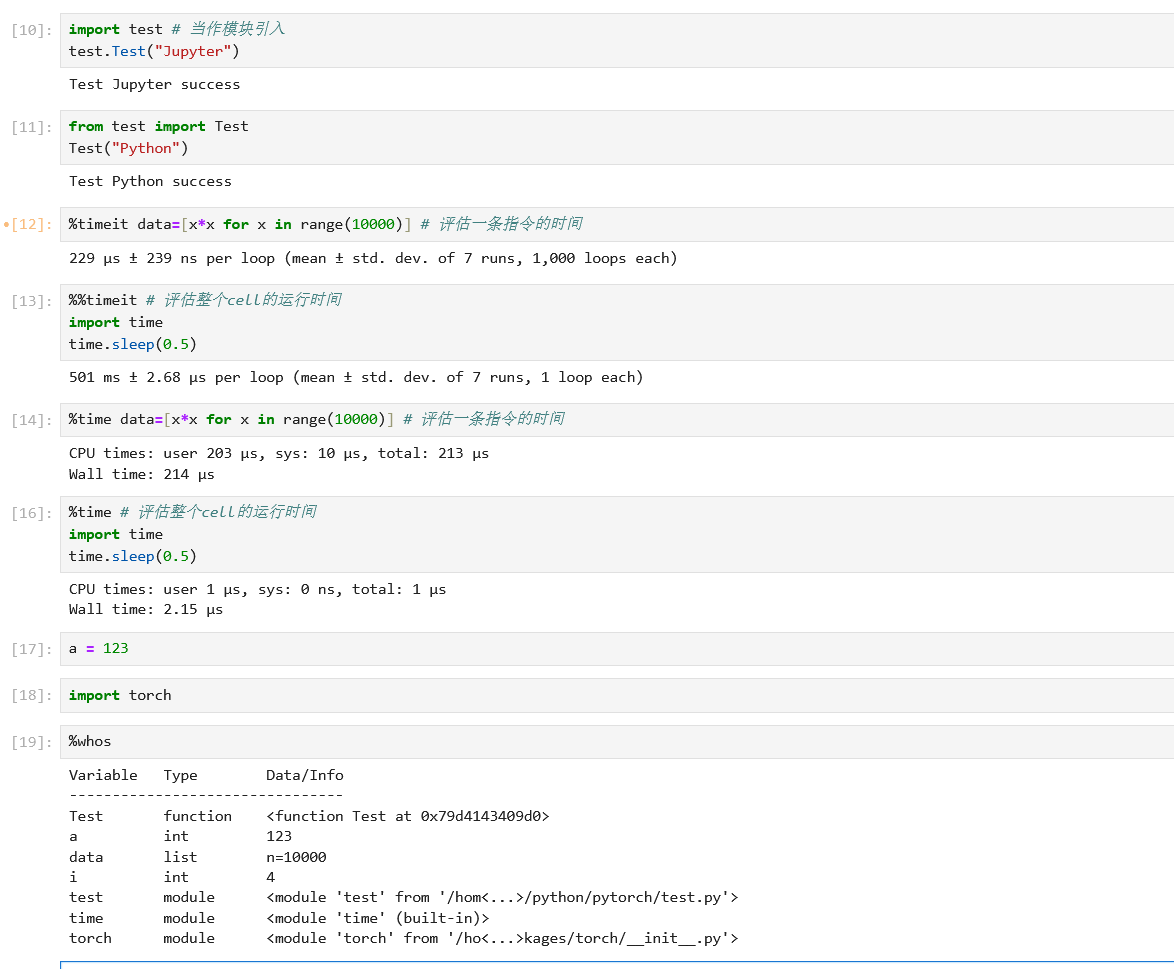
\includegraphics[width=0.8\textwidth]{part/软件工程/环境搭建/JupyterNotbook/pic/jupyternotebook语法/whos指令.png}
  \caption{whos指令}
  \label{fig:whos指令}
\end{figure}

\subsection{lsmagic 查看所有的魔法指令}
\begin{figure}[htpb]
  \centering
  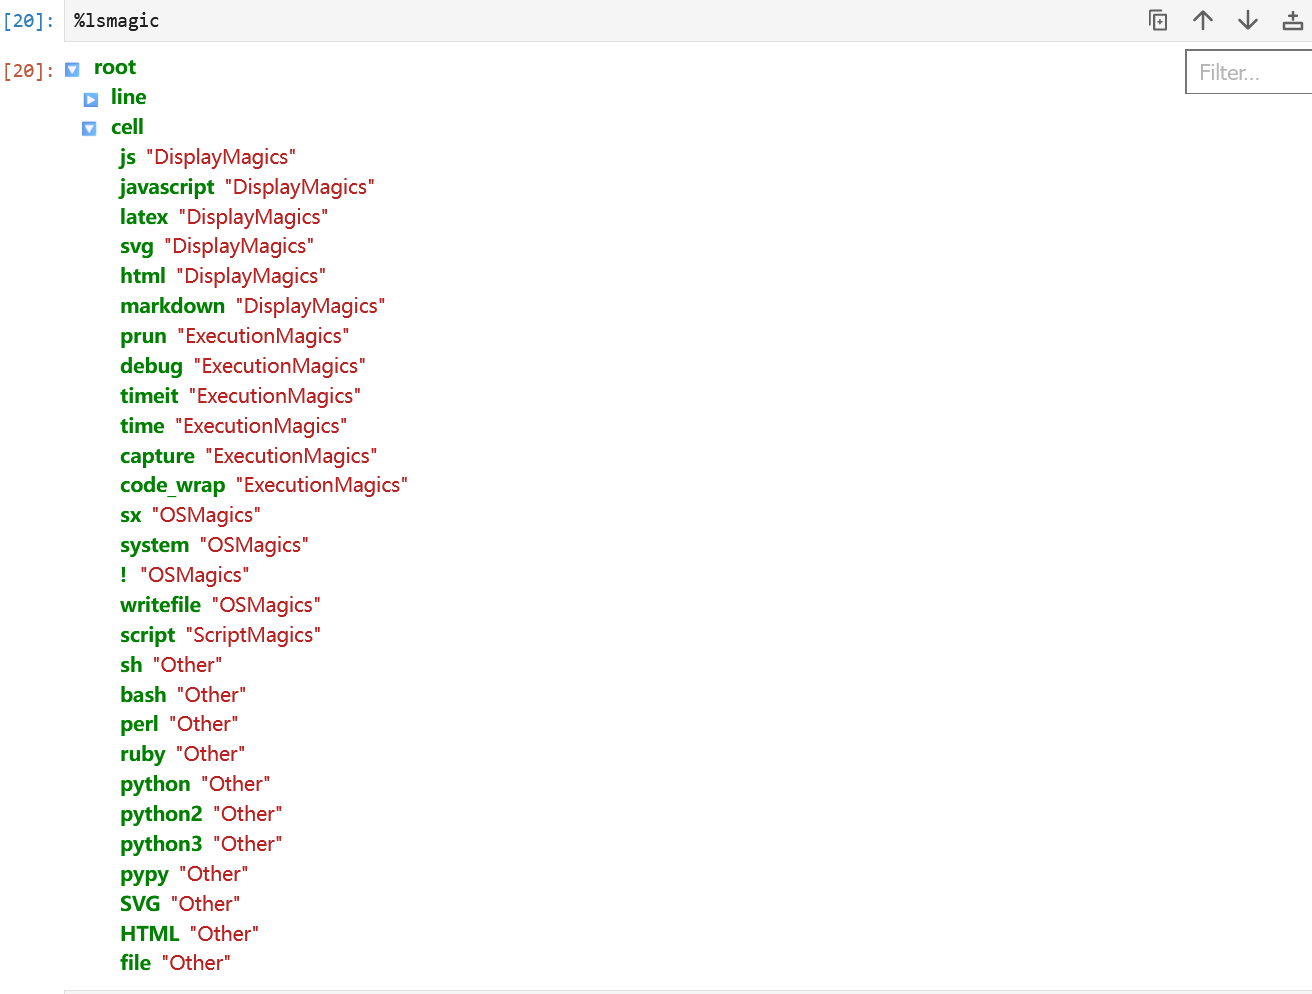
\includegraphics[width=0.8\textwidth]{part/软件工程/环境搭建/JupyterNotbook/pic/jupyternotebook语法/lsmagic指令.png}
  \caption{lsmagic指令}
  \label{fig:lsmagic指令}
\end{figure}




